\chapter{実装}
\label{chap:jissou}

本章では第\ref{chap:sekkei}章で述べたシステムの設計を受け、DrawWikiの実装について述べる。

\newpage

\section{アプリケーション構成}
DrawWikiはブラウザ上から利用できるWebアプリケーションとして実装されている。そのため
HTML5とSVG1.1に準拠したブラウザがインストールされていれば、OSやデバイスに依存せず利用することができる。
本アプリケーションの構成は以下の通りである。

\begin{figure}[htbp]
    \begin{center}
    {
\includegraphics[width=50mm]{images/testimage.png}} \end{center}
    \caption{アプリケーションの構成}
\end{figure}

\section{クライアントサイド}
実際にハイパーイラストを作成したり関連イラストを閲覧したりするクライアントサイドのプログラムはHTMLとjavascriptによって実装される。
開発にはJavascriptに変換可能な漸進的型付け言語TypeScriptを、UI操作ライブラリとしてReactをそれぞれ用いている。

\subsection{手書きデータの表現}
ブラウザに実装されているPointer-Events APIによって取得したイベントからパスのデータを生成し、描画する。
このAPIではマウスを含めてタッチやスタイラス等のあらゆるユーザー入力を透過的に扱うことができるため
あらゆる手書きデータ入力を受け付ける本システムで採用している。
このAPIはモダンなブラウザにはおおよそ搭載されているためプラットフォームを選ばずに利用できる。

\begin{figure}[htbp]
    \begin{center}
    {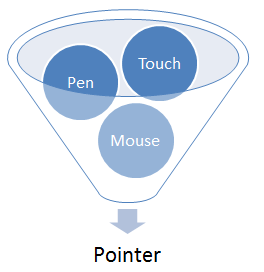
\includegraphics[width=50mm]{images/pevents.png}} \end{center}
    \caption{pointer-eventsの概要}
\end{figure}

\subsection{リンク付要素の視覚的表現}
関連イラスト表示にはリンクさせた、またはインポートしたハイパーイラストのサムネイルが表示される。
そのサムネイルを選択すると、そのハイパーイラストをリンクされている要素が強調表示される。
SVGはスタイルシートを読み込んで適用することもできるため、CSS/CSS transitionを用いて
この視覚的表現を実現している。

%\subsection{WYSIWYGエディタ}

\section{サーバーサイド}
Draw WikiはNode.js上で動作するWebアプリケーションとして実装されている。
HTTPリクエストを処理するWebアプリケーションフレームワークとしてExpressを用い、
そのホスティング環境としてBaaS(Backend-as-a-Service)の一つであるHerokuを利用している。

\subsection{ハイパーイラストのホスティング環境}
ファイルとしてのハイパーイラストはアプリケーションサーバーと異なる場所にホスティングされている。

